\section{Atrial Fibrillation Induced Remodelling And Heterogeneity}

The human atria consists of several tissue types each with distinct
electrophysiological properties.  It has previously been shown that
inhomogeneity in tissues can lead to re-entrant activity
\cite{Bernus2005, Coronel1992, Kumagai1997}.  There is also experimental
data available on the ion channel remodelling due to atrial
fibrillation induced remodelling (AFER) during chronic atrial
fibrillation (AF) on human atrial cells~\cite{Bosch1999,Workman2001}.
It is not known what effects electrophysiological remodelling caused by AF would
have on the natural heterogeneities present in the human tissue.
They might be augmented by the remodelling or reduced.
In addition, it is not known whether such changes in the heterogeneity are
anti- or pro-arrhythmogenic.

In this study, the changes induced by AFER were incorporated into cellular
models along with differences for the heterogeneity.
The APD and restitution behaviours of the cells were quantified and compared to
elucidate the influence of AFER on cell heterogeneity.
The modified cells were then incorporated into two dimensional electrically heterogeneous and
homogeneous models of the human atrium under different AFER conditions.
This was used to test whether the combination of AFER and heterogeneity was
anti- or pro-arrhythmogenic.

\subsection{Methods}

The human atrial action potential model by Courtemanche et
al.\cite{CRN98} was used in this study.  Modifications were
incorporated to reproduce the differing APs of the different atrial cell
types~\cite{Seemann2006}.  This produced distinct APs for the
crista terminalis (CT), pectinate muscles (PM), atrio-ventricular ring
bundle and the Bachmann bundle.  Atrial myocyte (AM) cells were modelled
by the original CRN model.

The data for AFER were taken from experiments by Bosch et
al.~\cite{Bosch1999} and Workman et al.~\cite{Workman2001}, representing
the changes in ion channels in patients after one month (Bosch)
and up to six months (Workman) of chronic AF, respectively.  The
modifications to the cellular electrophysiology were described in
Kharche et al.~\cite{Kharche2007}\ and reproduced in table~\ref{tbl:afer:params}.


\begin{table}
    \caption[Parameter modifications for AFER]{
       Parameter modifications to the unmodified CRN model to account for the
       electrophysiological remodelling of atrial myocytes.
       Two sets of parameter modifications are provided, to account for the
       experimental data collected by Bosch~et~al.~\cite{Bosch1999} and
       Workman~et~al.~\cite{Workman2001}.
       When percentages are given, they are up or down regulations compared to
       the magnitude of the current in the unmodified CRN model.
       The data from Bosch~et~al. also included at \mv{-16}\ shift in the steady
       state activation of \ii{to}\ and a \mv{+1.6}\ shift in the steady state
       activation of \ii{Na}.
    }
    \begin{center}
    \begin{tabular}{ l r r}
    \toprule
    Current & Bosch & Workman \\
    \midrule
    \ii{K1}   & $+235$\% & $+90$\% \\
    \ii{Ca,L} & $-74$\% & $-64$\% \\
    \ii{to}   & $-85$\% & $-65$\% \\
    \ii{Kur}  & --- & $+12$\% \\
    \ii{NaK}  & --- & $-12$\% \\
    $\tau_{\text{fCa}}$ & $+62$\% & --- \\
    \bottomrule
    \label{tbl:afer:params}
    \end{tabular}
    \end{center}
\end{table}

The effects of AFER were quantified through a variety of measures.  The
\apdr\ was calculated as described previously.
There were 10 S1 stimuli at a frequency of \unit{1}{Hz}, followed by a varying DI.
The ERP\emph{r} was calculated as described previously, with 10 S1 delivered at
the given pacing rate and then a final S2 stimulus was used to determine the ERP
after Workman et al.~\cite{Workman2001}.
The VW and the CV\emph{r} were determined for control,
Bosch and Workman conditions, for each of the three atrial cell types
considered.
There were therefore nine 1D strand models tested.  The strand
models were each 200 nodes long, with a spatial resolution of \mm{0.1}.  The
diffusion constant used for all simulations was set to
$0.03125\,\text{mm}^{\text{2}}\,\text{ms}^{\text{-1}}$~\cite{Biktasheva2005},
giving a solitary wave conduction velocity of
$0.267\,\text{mm}\,\text{ms}^{\text{-1}}$\ in control atrial tissue.  In all 1D
strand simulations there was 1 S1 pulse and one S2 pulse.  This pulse was
applied over 4 nodes (\unit{0.4}{mm}), had duration \ms{2} and magnitude
\unit{4}{nS}.
The higher stimulus strength was necessary to excite the AFER remodelled tissue.

Further, a 2D electrically heterogeneous sheet model was developed based on a
laboratory photograph of the right atrium.  The photograph was digitized at a
spatial resolution of \mm{0.1}. The model developed by segmenting areas of the
tissue into AM, PM and CT tissue types.  The complete model had an approximate size of
$130\times100\,\text{mm}$ and consisted of approximately 1 million active cell nodes.  The
simulations were performed with all cells under control, Bosch and Workman conditions,
with the conditions applied uniformly to the tissue.  All 2D sheet simulations
were performed with the space step of \mm{0.1} and a time step of \ms{0.05}.

\subsection{Results}

Simulations were performed for all three cases: control, Bosch and Workman.
However the results for Bosch and Workman were qualitatively similar, although
Bosch showed a much more profound effect on \apd\ reduction.

\begin{figure}
\centering
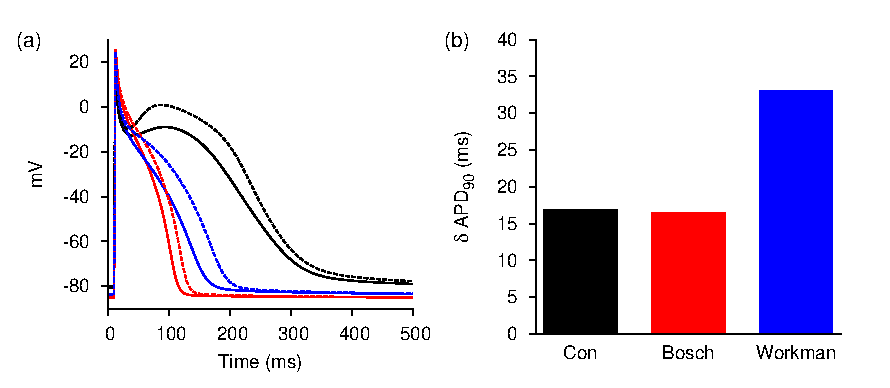
\includegraphics{figures/toolkit/afer/figures/01_APD}
\caption[AFER AP Plots And APD differences]{
\label{fig:toolkit:afer:apd}
(a).
Action potential profiles after pacing at \unit{1}{Hz}.
Results are shown for AM/PM cells (solid lines) and CT cells (dashed lines).
Control parameter traces are black, Bosch are red and Workman traces
blue.
The CT cells have a longer APD in all cases and show an elevated plateau
potential.
(b).
APD differences between AM/PM cells and CT cells after pacing at \unit{1}{Hz}.
Colour scheme as for panel (a).
There is almost no difference in $\delta$\apd\ between control and Bosch CT cells,
but $\delta$\apd\ increased markedly when Workman parameters are used.
}
\end{figure}

Incorporating the heterogeneity and AFER data causes significant differences in
\apd\ and AP morphology to manifest, as shown in
figure~\ref{fig:toolkit:afer:apd}(a).
The effects of AFER are not uniform across the different cell types of the
atrium in both cases (figure~\ref{fig:toolkit:afer:apd}(b)).
The difference in the AP between AM/PM myocytes and CT myocytes in the Workman
remodelled case is almost double that seen in either the Bosch remodelled case
or control case.
Note that in all cases there is almost no difference between AM and PM types.


\begin{figure}
\centering
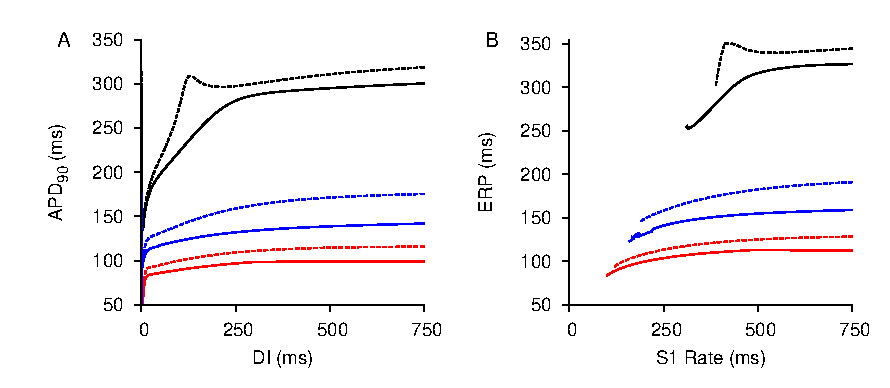
\includegraphics{figures/toolkit/afer/figures/02_APDR}
\caption[AFER APDr and ERPr curves]{
\label{fig:toolkit:afer:apdr}
(a)
\apdr\ curves showing \apd\ plotted against diastolic interval (DI) for control
(black), Bosch (red) and Workman (blue) cases.
AP/PM curves are shown as solid lines, CT curves are dashed.
AFER acts to flatten the restitution curves.
In all cases CT \apd\ is above AM/PM \apd.
(b)
ERP\emph{r}\ curves showing ERP plotted against S1 interval.
Colour scheme is as for panel (a).
In all cases CT ERP is above AM/PM ERP.
Note that AFER enables successful excitation at much lower S1 intervals.
}
\end{figure}

The \apdr\ curves, shown in figure~\ref{fig:toolkit:afer:apdr}(a), are
flatter over much of the range of diastolic intervals for Bosch and Workman as
compared to control.
The curves have two clear phases in the AFER cases; a very steep initial rise
and then slower, asymptotic rise in \apd.
In the control case the curves show an intermediate a phase with a slope between
the two extremes.
In the control CT case, the curves include a prominent notch at a DI of
approximately \ms{130}\ which is caused by the up regulation of \ii{Ca,L}\ in CT
cells.
The down regulation associated with the AFER removes this.
In both of the AFER cases, the curves are almost flat at DI \ms{750}, but in the
control case, the \apd\ is still rising.
The figure also emphasises the increased heterogeneity observed in the Workman
case.

In AF tissue, the ERP\emph{r} was flattened for all tissue types compared with
the control cells, as shown in figure~\ref{fig:toolkit:afer:apdr}(b).
The curves also extended to lower S1 intervals for AF tissue, indicating that it
was possible to excite AF tissue successfully at a higher rate than was possible
in control tissue.
Heterogeneity in ERP\emph{r} was largely unaffected by AF.

\begin{figure}
\centering
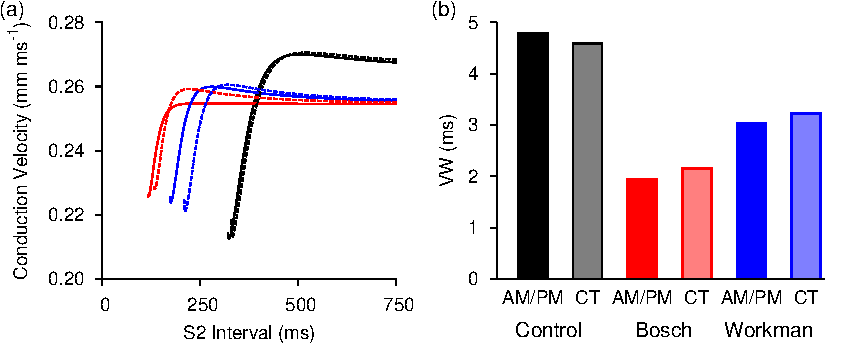
\includegraphics{figures/toolkit/afer/figures/03_CVR}
\caption[AFER CVr curves and VWs]{
\label{fig:toolkit:afer:cvr}
(a) 
CV\emph{r}\ curves for Control (black), Bosch (red) and Workman (blue) tissues.
AM/PM cells are indicated by solid lines, CT cells by dashed.
In all cases CT cells show a higher conduction velocity at long
($>$\ms{600}) S2 intervals, but AM/PM muscles allow faster conduction at lower
S2 intervals.
AF cases show a reduced CV in all instances and support
higher pacing rates via reduced minimal interval.
(b) Vulnerability Window for Control (black), Bosch (red) and Workman (blue).
AM/PM cell types are shown solid, CT are partially shaded.
The VW is reduced for the AF remodelled cases via reduced excitability.
The presence of the remodelling also reverses the difference in VW between cell
types.
}
\end{figure}

Conduction velocity, shown in figure~\ref{fig:toolkit:afer:cvr}(a), was slowed by AF,
reducing the solitary wave velocity from $0.27\,\text{mm}\,\text{ms}^{\text{-1}}$\ in
control to $0.25\,\text{mm}\,\text{ms}^{\text{-1}}$\ in Bosch and
$0.26\,\text{mm}\,\text{ms}^{\text{-1}}$\ in
Workman.
Maximal pacing rate increased from the control value of \unit{187}{bpm} to
\unit{512}{bpm} in Bosch strands and \unit{347}{bpm} in Workman strands of AM or
PM cells.
In CT strands, maximal pacing rates of \unit{183}{bpm}, \unit{451}{bpm}\ and
\unit{287}{bpm}\ were observed for Control, Bosch and Workman cases
respectively.
The heterogeneity of minimal pacing intervals is significantly increased by
AFER, from \unit{4}{bpm}\ to over \unit{50}{bpm}\ in Bosch and Workman strands.

The VW was reduced by AF, figure~\ref{fig:toolkit:afer:cvr}(b).
The control value of \ms{4.8}\ was reduced to \ms{2.0}\ in Bosch and \ms{3.0}\ in Workman for AM and PM cell types.
In CT cells under control conditions, the VW was reduced to \ms{}
The reduction in VW for CT cells was reduced, to \ms{4.6}.
In contrast, the VW increased for AF cases; \ms{2.1}\ and \ms{3.2}\ for Bosch
and Workman cases respectively.


\begin{figure}
\centering
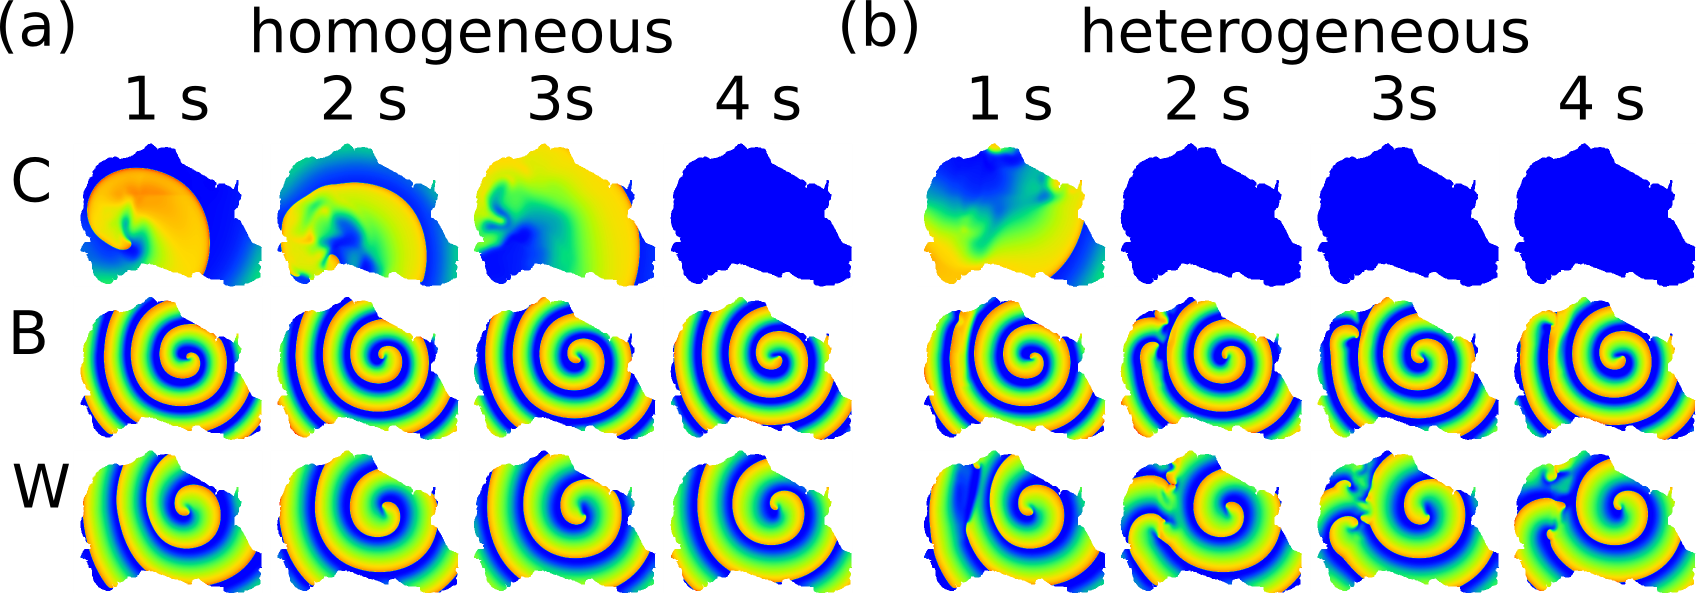
\includegraphics{figures/toolkit/afer/2d_plots}
\caption[AFER 2D re-entry plots]{
\label{fig:toolkit:afer:2d}
Simulation of re-entry in 2D sheets of electrically homogeneous
(a) and electrically heterogeneous (b) sheets.
Colour represents membrane potential from blue (resting) to orange (excited).
Columns show representative frames after initiation of re-entry at t = 0.
Rows C, B, W show data from control, Bosch and Workman cases, respectively.
Re-entry self-terminated under control conditions in both homogeneous (a)(C) and
heterogeneous (a)(C).
Under AF conditions, re-entry becomes a sustained mother rotor in
electrically homogeneous conditions ((a)(B), (a)(W)).
However, under electrically heterogeneous conditions AF causes re-entry to degenerate
into erratic propagations on the borders of the heterogeneity ((b)(B), (b)(W)) }
\end{figure}

Simulations over the 2D geometry examined the lifetime and behaviour of
spiral waves in the presence and absence of electrical heterogeneity.
As can be seen in figure~\ref{fig:toolkit:afer:2d}, panels (a)(C) and (b)(C), re-entrant
activity self-terminated in both homogeneous and heterogeneous cases.
Spiral wave meander over a large region of tissue eventually causes the tip to
leave the tissue.
Self-termination was much more rapid in the electrically heterogeneous case,
taking \unit{1.31}{s}, compared with \unit{3.20}{s} in the homogeneous case.

Conversely, under AF conditions the re-entry persisted after it was
induced for the whole period of the simulation, a lifespan of over \unit{5}{s}.
Under electrically homogeneous conditions, panels (a)(B) and (a)(W) show a
stable mother rotor rotating anti-clockwise in the tissue.
In heterogeneous conditions, as shown in panels (b)(B) and (b)(W), a similar
mother rotor to the homogeneous cases is visible towards the right of each
frame.
On the left of the frames, the rotor breaks up into multiple fibrillatory
wavelets on the border of the heterogeneous regions, forming a complex and
chaotic pattern of excitation.


\subsection{Discussion and conclusions}

AFER induces significant changes in the cellular electrophysiology that
appear to affect rate dependent electrical activities.  It helps to
sustain re-entry, providing evidence to substantiate the hypothesis of
`AF begets AF'.

The single cell results show a striking reduction in the \apd\ and
repolarization properties.
AFER abbreviated \apd\ in AM cells by 66~\% in Bosch and 53~\% in Workman.
Other work~\cite{Xie2002,ByungSoo2002,Karma1994,Tusscher2006} has already suggested why flattening of
the ERP and APD restitution curves can be pro-arrhythmogenic.
Our study suggested that reduction is not uniform across all cell types, which
leads to an augmented heterogeneity.

From the 1D results, AFER tissue forms a much better substrate for arrhythmic
activity.
It supports a much higher pacing rate and has a reduced conduction wavelength
(conduction velocity multiplied by \apd), allowing a greater number of
excitation waves to exist in the tissue.
The increase in the heterogeneity of the maximal pacing rates suggests that
remodelled tissues might be more vulnerable to localised regions of conduction
block.
This has been shown to lead to re-entry~\cite{Xie2001a}.

The 2D simulations in the realistic sheet show a marked difference in
re-entrant behavior between homogeneous and heterogeneous simulations.
The homogeneous sheets show self-termination of re-entry in control
tissue, whilst the reduced ERP and conduction wavelength allow the rotor
to remain stable and persist for the duration of the simulation in AFER
condtions as is expected from the flattened restitution
curves~\cite{Xie2002,Karma1994}.
The heterogeneous sheet simulations, show spiral wave
breakup, as observed in real tissue \cite{Kumagai1997}, in both control
and AF simulations, possibly due to elevated plateau potentials and
increased refractory period of the CT cells~\cite{Clayton2005}, combined with
the slower conduction velocity at high pacing rates.
Self-termination is still observed in control simulations and is more rapid than
in homogeneous tissue.

It is still unclear about the pro- or anti-arrhythmogenic effects of
electrical heterogeneity in the human atria.  Self-termination is more
rapid in the heterogeneous tissue for the control case, but despite AFER
increasing the heterogeneity between tissue types, it doesn't lead to
self termination of the re-entry.  In fact, it leads to breakup of the
spiral wave in the region of the heterogeneity, leading to a region of
erratic propagations, as has been seen in experiment~\cite{Kumagai1997}.
Further study, in both 3D geometries and physiological experiments,
would be needed to elucidate the true effects of the heterogeneity.
